\subsubsection{Functional Requirements}
\begin{itemize}
  \item The system shall kwon if a car is avaible or not.
  \item The system shall know if an user is already reserving a car.
  \item The system shall turn a car avaible or not avaible.
  \item The system shall know the time when an user do a reservation.
  \item The system shall tag a car avaible again if a car is not picked-up within an hour from the reservation.
\end{itemize}

\subsubsection{Scenario 1}
Mark needed to go to the city center and he decided to use a PowerEnJoy's car. He has checked online that there is an avaible car near his position but before to go he would have a quick lunch. He wanted to be sure than after his lunch the car would be still avaible so he decided to reserve the car.
Unexpectedly Morgan, a friend of Lucas, decided to go to have lunch in the same place of Mark. When they saw each other they were very happy and they started to chat about their jobs. When they finished to talk Mark notice that PowerEnJoy sent him an e-mail. The mail was about his reservation that expired due to the fact the the hour was finished. His bank has also notified him that a fee of 1€ was applied by PowerEnJoy.


\subsubsection{Scenario 2}
Susan is a typical PowerEnJoy user, she was walking through a street when a friend texts her to hang out. Fortunately she saw a PowerEnJoy's car on the other side of the street. She reached the car and checked online: that's not available. Someone had probably already reserved it. But on the app she noticed that there were two avable car 5 minutes walk from her position. Than she reserved one of that two cars and easily reached it, thanks to the accurate location service provided by the system. 


\subsubsection{Mockups}
\begin{figure}[!ht]
  \centering
  \vspace{0.1cm}
  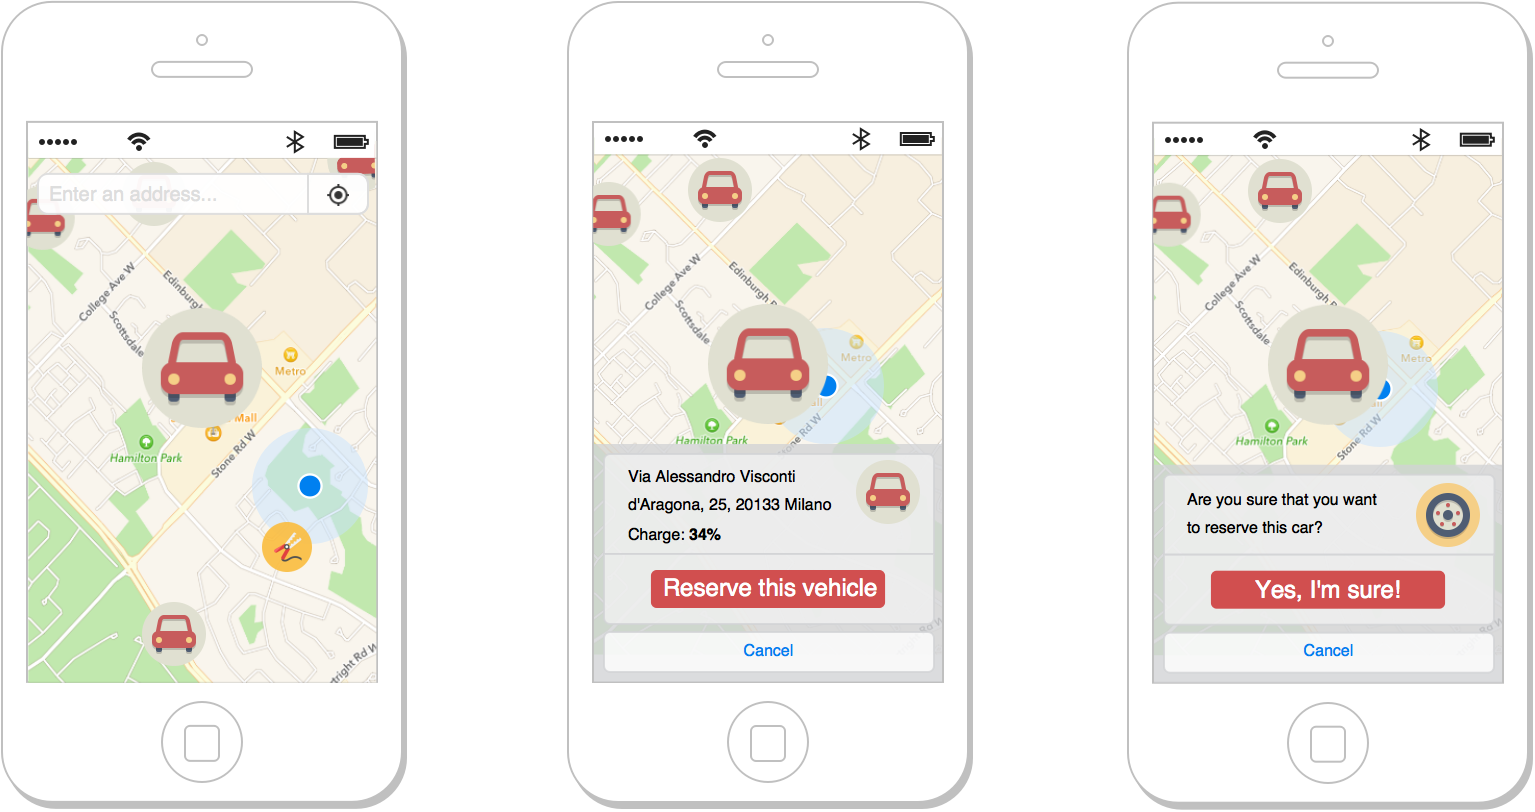
\includegraphics[width=1\textwidth]{/RASD/System_Functions/create_reservation_mockup}\\
  \vspace{0.4cm}
  %\caption{Mockup for the login mobile page} 
  \label{fig:create_reservation_mockup} 
\end{figure}
% maybe home page mockup here 


\subsubsection{Use-case table}
\begin{center}
  \begin{tabular}{ l | p{10cm} }
    \hline
    Actors & Guest\\ \hline
    Goal & G\ref{itm:goal-reservation}\\ \hline
    Entry conditions & \begin{itemize}
			\item The User is in his homepage and want to reserve a car.
			\item PowerEnJoy has available cars.
			\item The User is not already reserving a car.
\end{itemize}  \\ \hline
    Flow of events &
\begin{itemize}
%\item The User select the "Find a car" option.
\item The User has three ways for finding a car:
\begin{itemize}
			\item browse the map.
			\item use her location.
			\item enters an address.
\end{itemize}
%\item The system loads a map of the selected area and the avaible cars' locations near there .
\item The User selects the car that want to reserve.
\item the system displays the car's information.%Maybe to add to the mockup
%\item The User presses the "Yes,I'm sure" button for confirm the reservation.
\item The system turn the car "reserved".% and start the reservation timer.
\item The system notified the User.
\end{itemize} \\ \hline
    Exit conditions &
\begin{itemize}
	\item A car is set as "reserved".
	\item The car is reserved for up one hour. After that the reservation expires and the User has to pay a fee of 1€.
\end{itemize}  \\ \hline
  Exceptions & 
%\begin{itemize}
%\item The User has already reserved a car.

%\item 
The system is not able to complete the operation due to some internal issues or connection broken (the system signals a ConnectionFailure).%volendo si possono modificare i nomi delle eccezzioni.
%\end{itemize} 
\\ \hline
  \end{tabular}
\end{center}


\subsubsection{Sequence diagram}
\begin{figure}[!ht]
  \centering
  \vspace{0.2cm}
  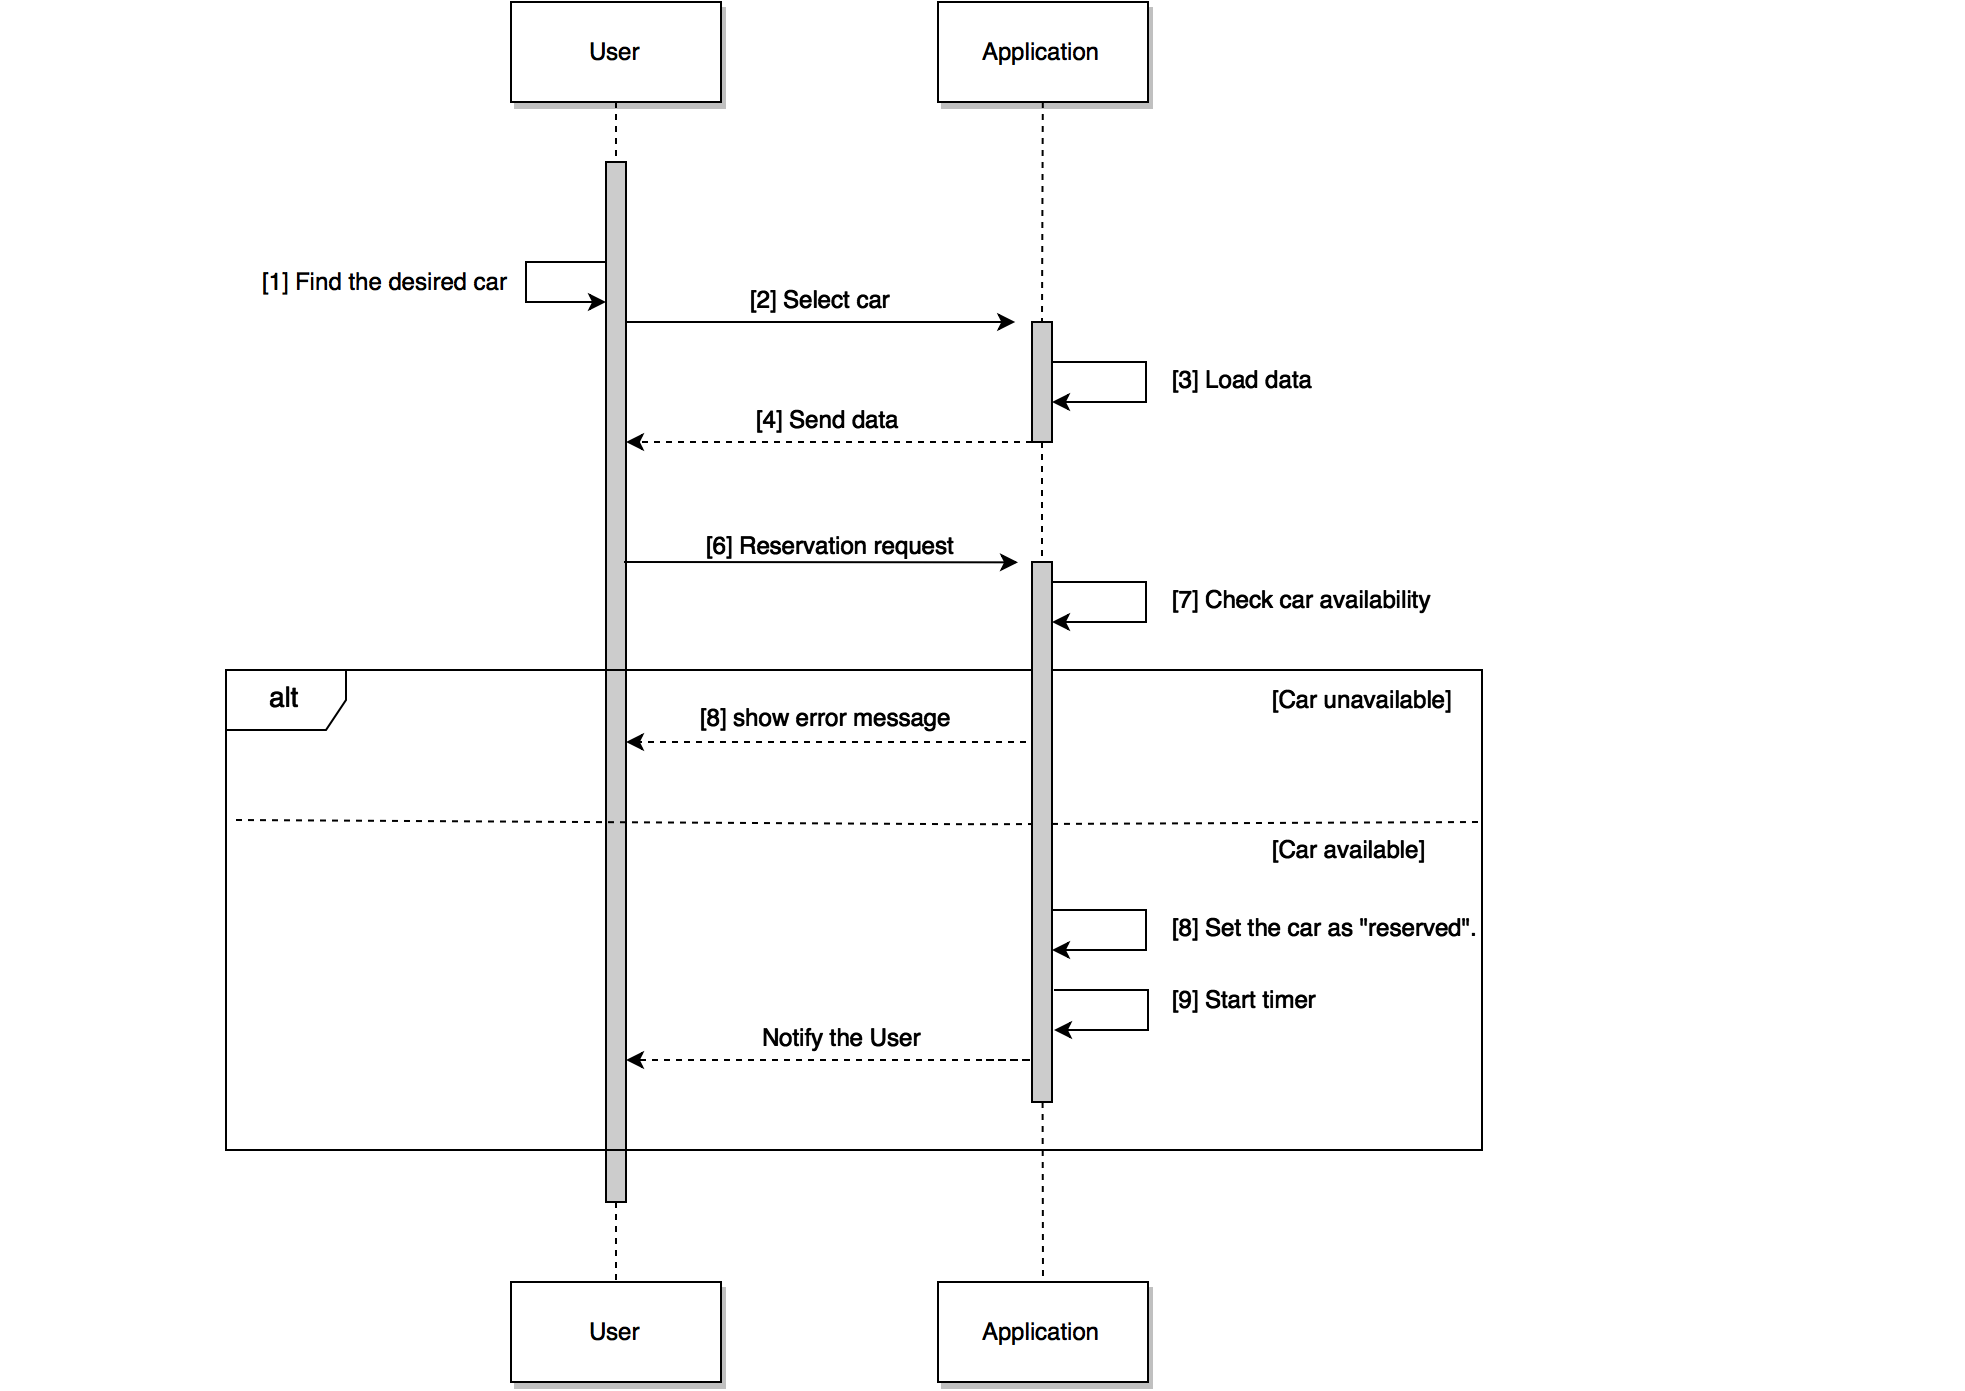
\includegraphics[width=1.2\textwidth]{/RASD/System_Functions/reservation_sequence}\\
  \vspace{0.1cm}
  %\caption{Sequence diagram for the login procedure} 
  \label{fig:reservation_sequence} 
\end{figure}

